\renewcommand{\theequation}{\theenumi}
\begin{enumerate}[label=\arabic*.,ref=\thesubsection.\theenumi]
\numberwithin{equation}{enumi}

\item The vector equation for the conic is
\begin{align}
\vec{x}^T\myvec{1 & 0\\0 & 0}\vec{x} + \myvec{-2 & 0}\vec{x} -8 = 0
\\
x^2-2x-8 = 0
\\
\left(x-4\right)\left(x+2\right) = 0
\\
 \alpha = 4 ,\beta =-2 
\end{align}
quadratic equation can be represented as 
\begin{align}
ax^2+bx +c = 0
\\
\alpha +\beta = -\frac{b}{a} = 2
\\
\alpha \times \beta = \frac{c}{a} = -8
\end{align}

\begin{figure}[!ht]
	\centering
	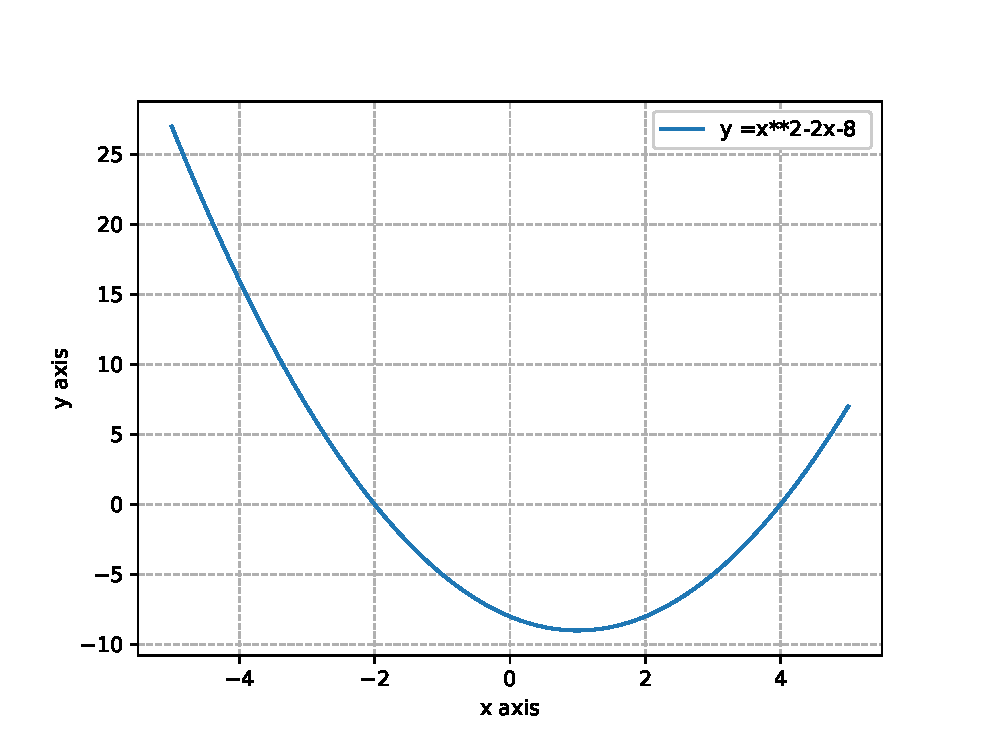
\includegraphics[width=\columnwidth]{./solutions/4/figures/conics/perabola1.eps}
	\caption{}
	\label{fig:5.2.3_perabola1}
\end{figure}
\begin{lstlisting}
solutions/4/codes/conics/perabola2.py
\end{lstlisting}


\item The vector equation for the conic is
\begin{align}
\vec{x}^T\myvec{4 & 0\\0 & 0}\vec{x} + \myvec{8 & 0}\vec{x} = 0
\\
4u^2 + 8u = 0
\\
\left(4u\right)\left(u+2\right) = 0
\\
\alpha = 0 ,\beta =-2 
\end{align}
quadratic equation can be represented as 
\begin{align}
ax^2+bx +c = 0
\\
\alpha +\beta = -\frac{b}{a} = -2
\\
\alpha \times \beta = \frac{c}{a} = 0
\end{align}
\begin{figure}[!ht]
	\centering
	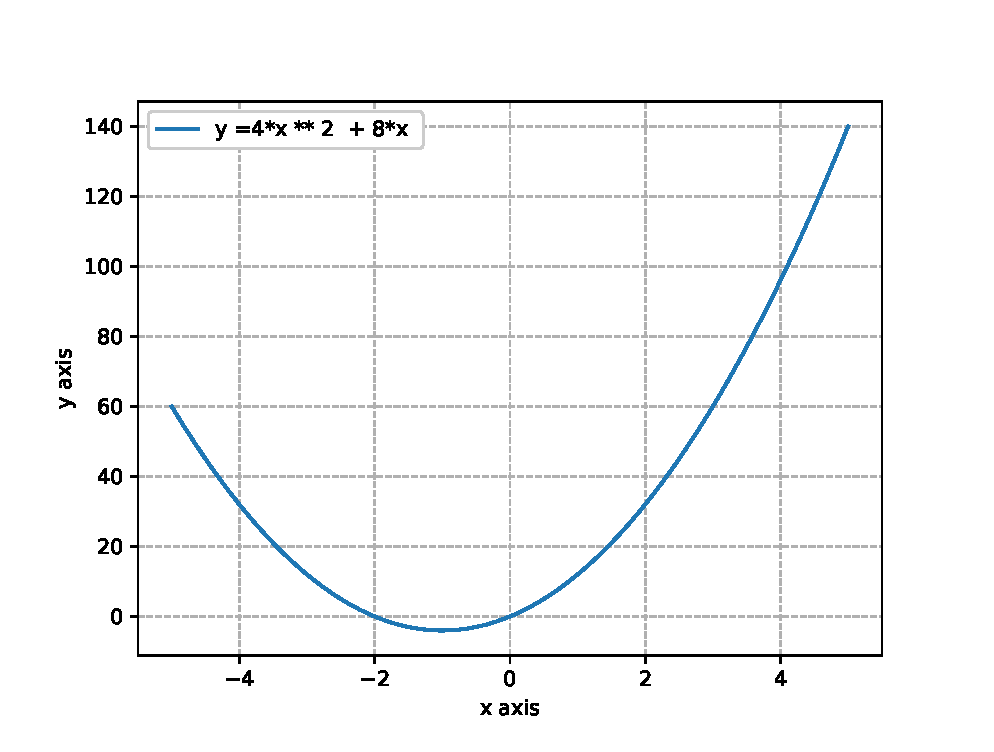
\includegraphics[width=\columnwidth]{./solutions/4/figures/conics/perabola2.eps}
	\caption{equation 2 }
	\label{fig:5.2.3_perabola2}
\end{figure}
\begin{lstlisting}
solutions/4/codes/conics/perabola2.py
\end{lstlisting} 

\item The vector equation for the conic is
\begin{align}
\vec{x}^T\myvec{4 & 0\\0 & 0}\vec{x} + \myvec{-4 & 0}\vec{x} +1 = 0
\\
4s^2-4s+1 = 0
\\
\left(2s-1\right)\left(2s - 1\right) = 0
\\
\alpha = \frac{1}{2} ,\beta =-\frac{1}{2} 
\end{align}
quadratic equation can be represented as 
\begin{align}
ax^2+bx +c = 0
\\
\alpha +\beta = -\frac{b}{a} = 1
\\
\alpha \times \beta = \frac{c}{a} = \frac{1}{4}
\end{align}
\begin{figure}[!ht]
	\centering
	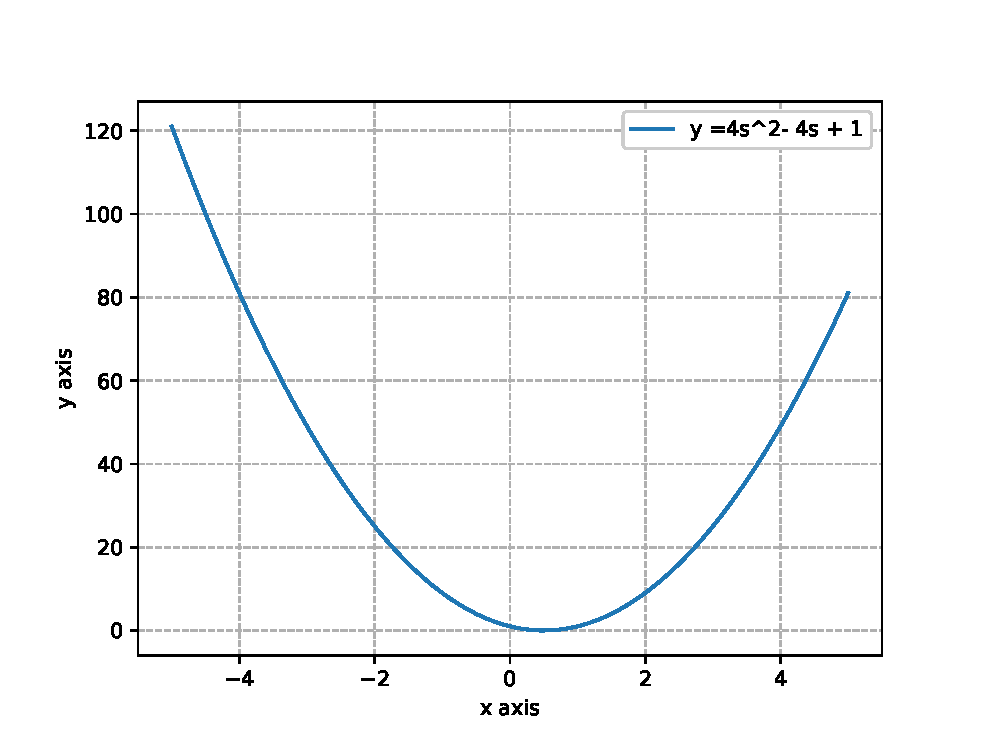
\includegraphics[width=\columnwidth]{./solutions/4/figures/conics/perabola3.eps}
	\caption{equation 3 }
	\label{fig:5.2.3_perabola3}
\end{figure}
\begin{lstlisting}
solutions/4/codes/conics/perabola3.py
\end{lstlisting}

\item The vector equation for the conic is
\begin{align}
\vec{x}^T\myvec{1 & 0\\0 & 0}\vec{x} + \myvec{0 & 0}\vec{x} -15= 0
\\
t^2 - 15 = 0
\\
\alpha = \sqrt {15} ,\beta =-\sqrt {15} 
\end{align}
quadratic equation can be represented as 
\begin{align}
ax^2+bx +c = 0
\\
\alpha +\beta = -\frac{b}{a} = 0
\\
\alpha \times \beta = \frac{c}{a} = -15
\end{align}
\begin{figure}[!ht]
	\centering
	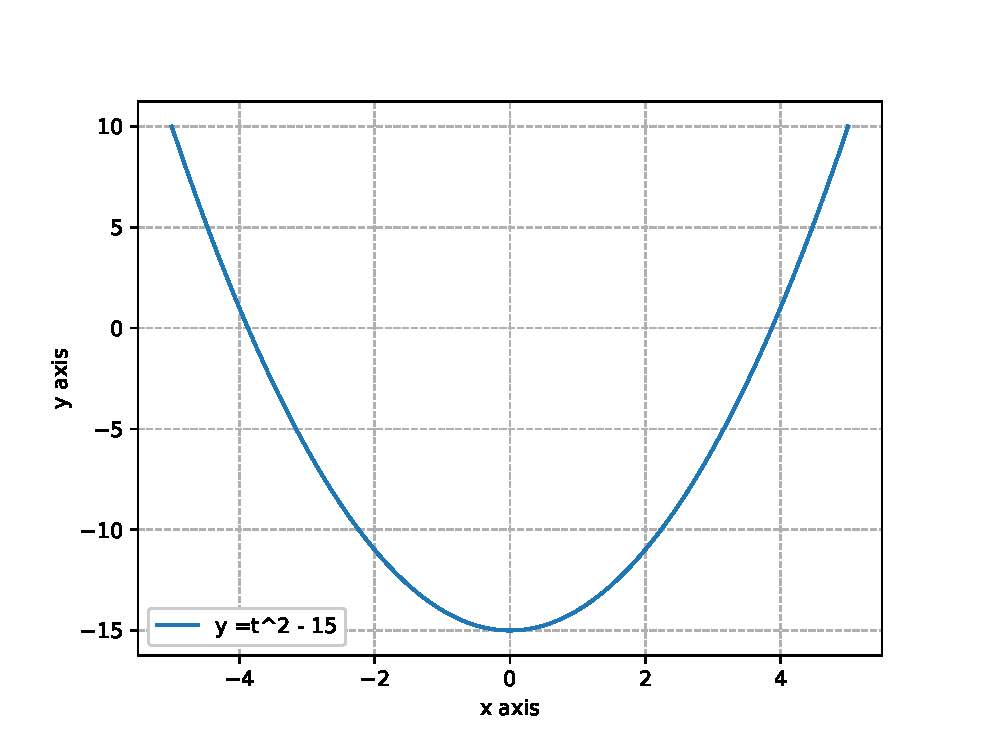
\includegraphics[width=\columnwidth]{./solutions/4/figures/conics/perabola4.eps}
	\caption{equation 4 }
	\label{fig:5.2.3_perabola4}
\end{figure}
\begin{lstlisting}
solutions/4/codes/conics/perabola4.py
\end{lstlisting}

\item The vector equation for the conic is
\begin{align}
\vec{x}^T\myvec{6 & 0\\0 & 0}\vec{x} + \myvec{-7 & 0}\vec{x} -3= 0
\\
6x^2-3-7x = 0
\\
\left(2x - 3\right)\left(3x\ + 1\right) = 0
\\
\alpha = \frac{3}{2},\beta =-\frac{1}{3}
\\
\alpha +\beta = -\frac{b}{a} = \frac{7}{6}
\\
\alpha \times \beta = \frac{c}{a} = -\frac{1}{2}
\end{align}
	\begin{figure}[!ht]
	\centering
	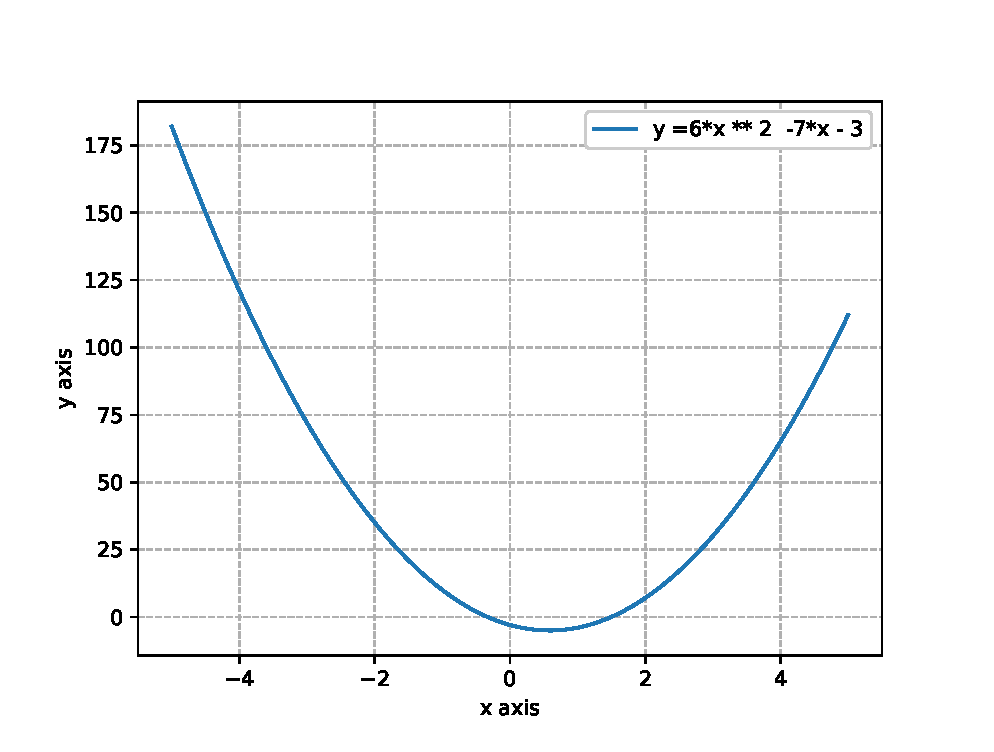
\includegraphics[width=\columnwidth]{./solutions/4/figures/conics/perabola5.eps}
	\caption{equation 5 }
	\label{fig:5.2.3_perabola5}
\end{figure}
\begin{lstlisting}
solutions/4/codes/conics/perabola5.py
\end{lstlisting}

\item The vector equation for the conic is
\begin{align}
\vec{x}^T\myvec{3 & 0\\0 & 0}\vec{x} + \myvec{-1 & 0}\vec{x} -4= 0
\\
3x^2-2x-8 = 0
\\
\left(3x + 4\right)\left(x + 1\right) = 0
\\
\alpha = -1,\beta =-\frac{4}{3}
\end{align}

\begin{figure}[!ht]
	\centering
	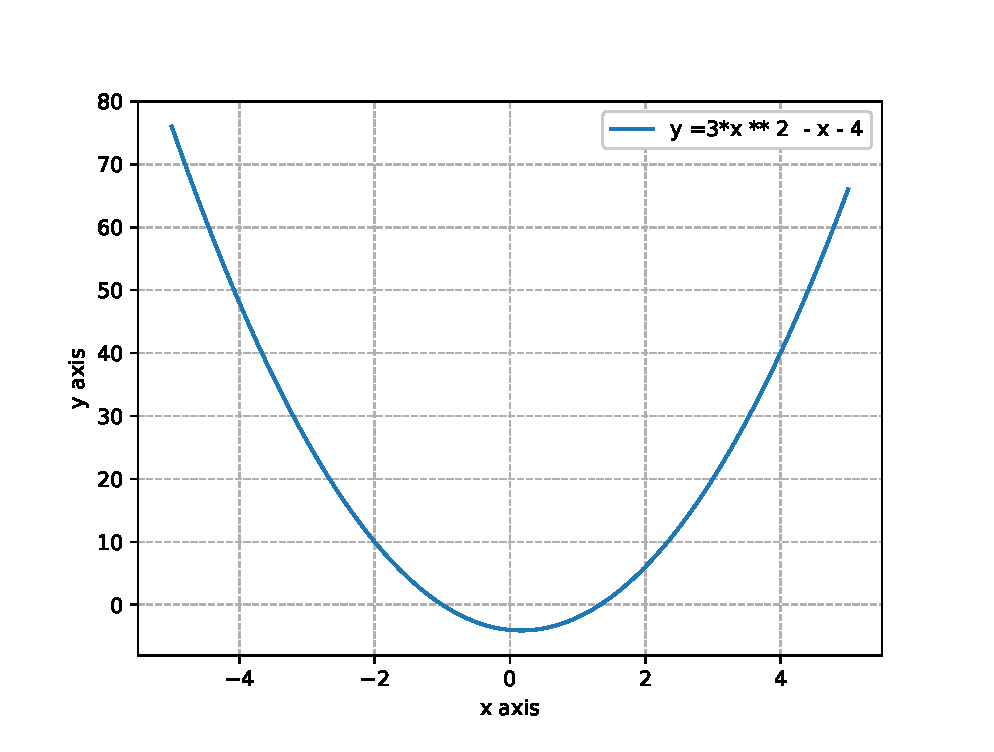
\includegraphics[width=\columnwidth]{./solutions/4/figures/conics/perabola6.eps}
	\caption{equation 6 }
	\label{fig:5.2.3_perabola6}
\end{figure}
\begin{lstlisting}
solutions/4/codes/conis/perabola6.py
\end{lstlisting}
quadratic equation can be represented as 
\begin{align}
ax^2+bx +c = 0
\\
\alpha +\beta = -\frac{b}{a} = \frac{2}{3}
\\
\alpha \times \beta = \frac{c}{a} = -\frac{8}{3}
\end{align}

\end{enumerate}
